\documentclass[12pt]{article}

\usepackage{mathptmx}  
\usepackage[T1]{fontenc}
\usepackage[utf8]{inputenc}
\usepackage[english]{babel}

% Page layout settings
\usepackage[margin=1.87cm]{geometry}

% Line spacing
\usepackage{setspace}
\setstretch{1.0}

% Paragraph formatting
\usepackage{parskip}
\usepackage{ragged2e}
\usepackage{wrapfig}
\RaggedRight 
\usepackage{float}
\usepackage{graphicx}
\usepackage{fancyhdr}
% For references
\usepackage[square,numbers]{natbib}

\pagestyle{fancy}
\fancyhf{} % clear header/footer
\fancyhead[R]{Xiaomao Wang} % name on right side
\fancyfoot[C]{\thepage}
\renewcommand{\headrulewidth}{0pt}

\begin{document}
\section*{Growth and Reproductive Trade-offs in Mast-Seeding Trees}
\textbf{Context} The fundamental processes in a plant’s life cycle—growth, reproduction, defense—all compete for the same resources \citep{bazzaz1997plant}, leading to trade-offs that maximize plant fitness when resources are limited. One key trade-off is the growth-reproduction trade-off \citep{grime1977evidence, stearns1998evolution}, which leads to high variability in reproduction across years. This is manifested as mast seeding, the phenomenon of synchronized variable seed production within plant populations \citep{kelly1994evolutionary, kelly2002mast, koenig2021brief, pearse2016mechanisms}.

Mast seeding plays a critical role in forest dynamics. It directly affects forest recruitment by increasing seed survival rates during mast years due to synchronized big seed crops \citep{bogdziewicz2020flowering, crone2014resource, silvertown1980evolutionary}. It also indirectly regulates populations of seed predators and pathogens by creating cycles of satiation and starvation \citep{davies2024seed, janzen1971seed}. This strategy not only improves short-term seedling survival but also promotes long-term forest regeneration, helping to maintain sustainable forest ecosystems over time. However, due to the fact that certain environmental factors are related to trigger masting, and altered resource availability due to less predictable changing climate, it is more and more difficult to predict how masting pattern is going to change. It is important to understand how trees allocate resource between growth and reproduction and how to tease apart environmental effects on them separately to to help us build a robust model. This allocation has broader implications for forest productivity and the global carbon cycle, depending on whether additional carbon is invested in wood growth or seed production.

\setlength{\columnsep}{2pt}
\setlength{\intextsep}{2pt}

\begin{wrapfigure}{r}{0.65\textwidth}
    \centering
    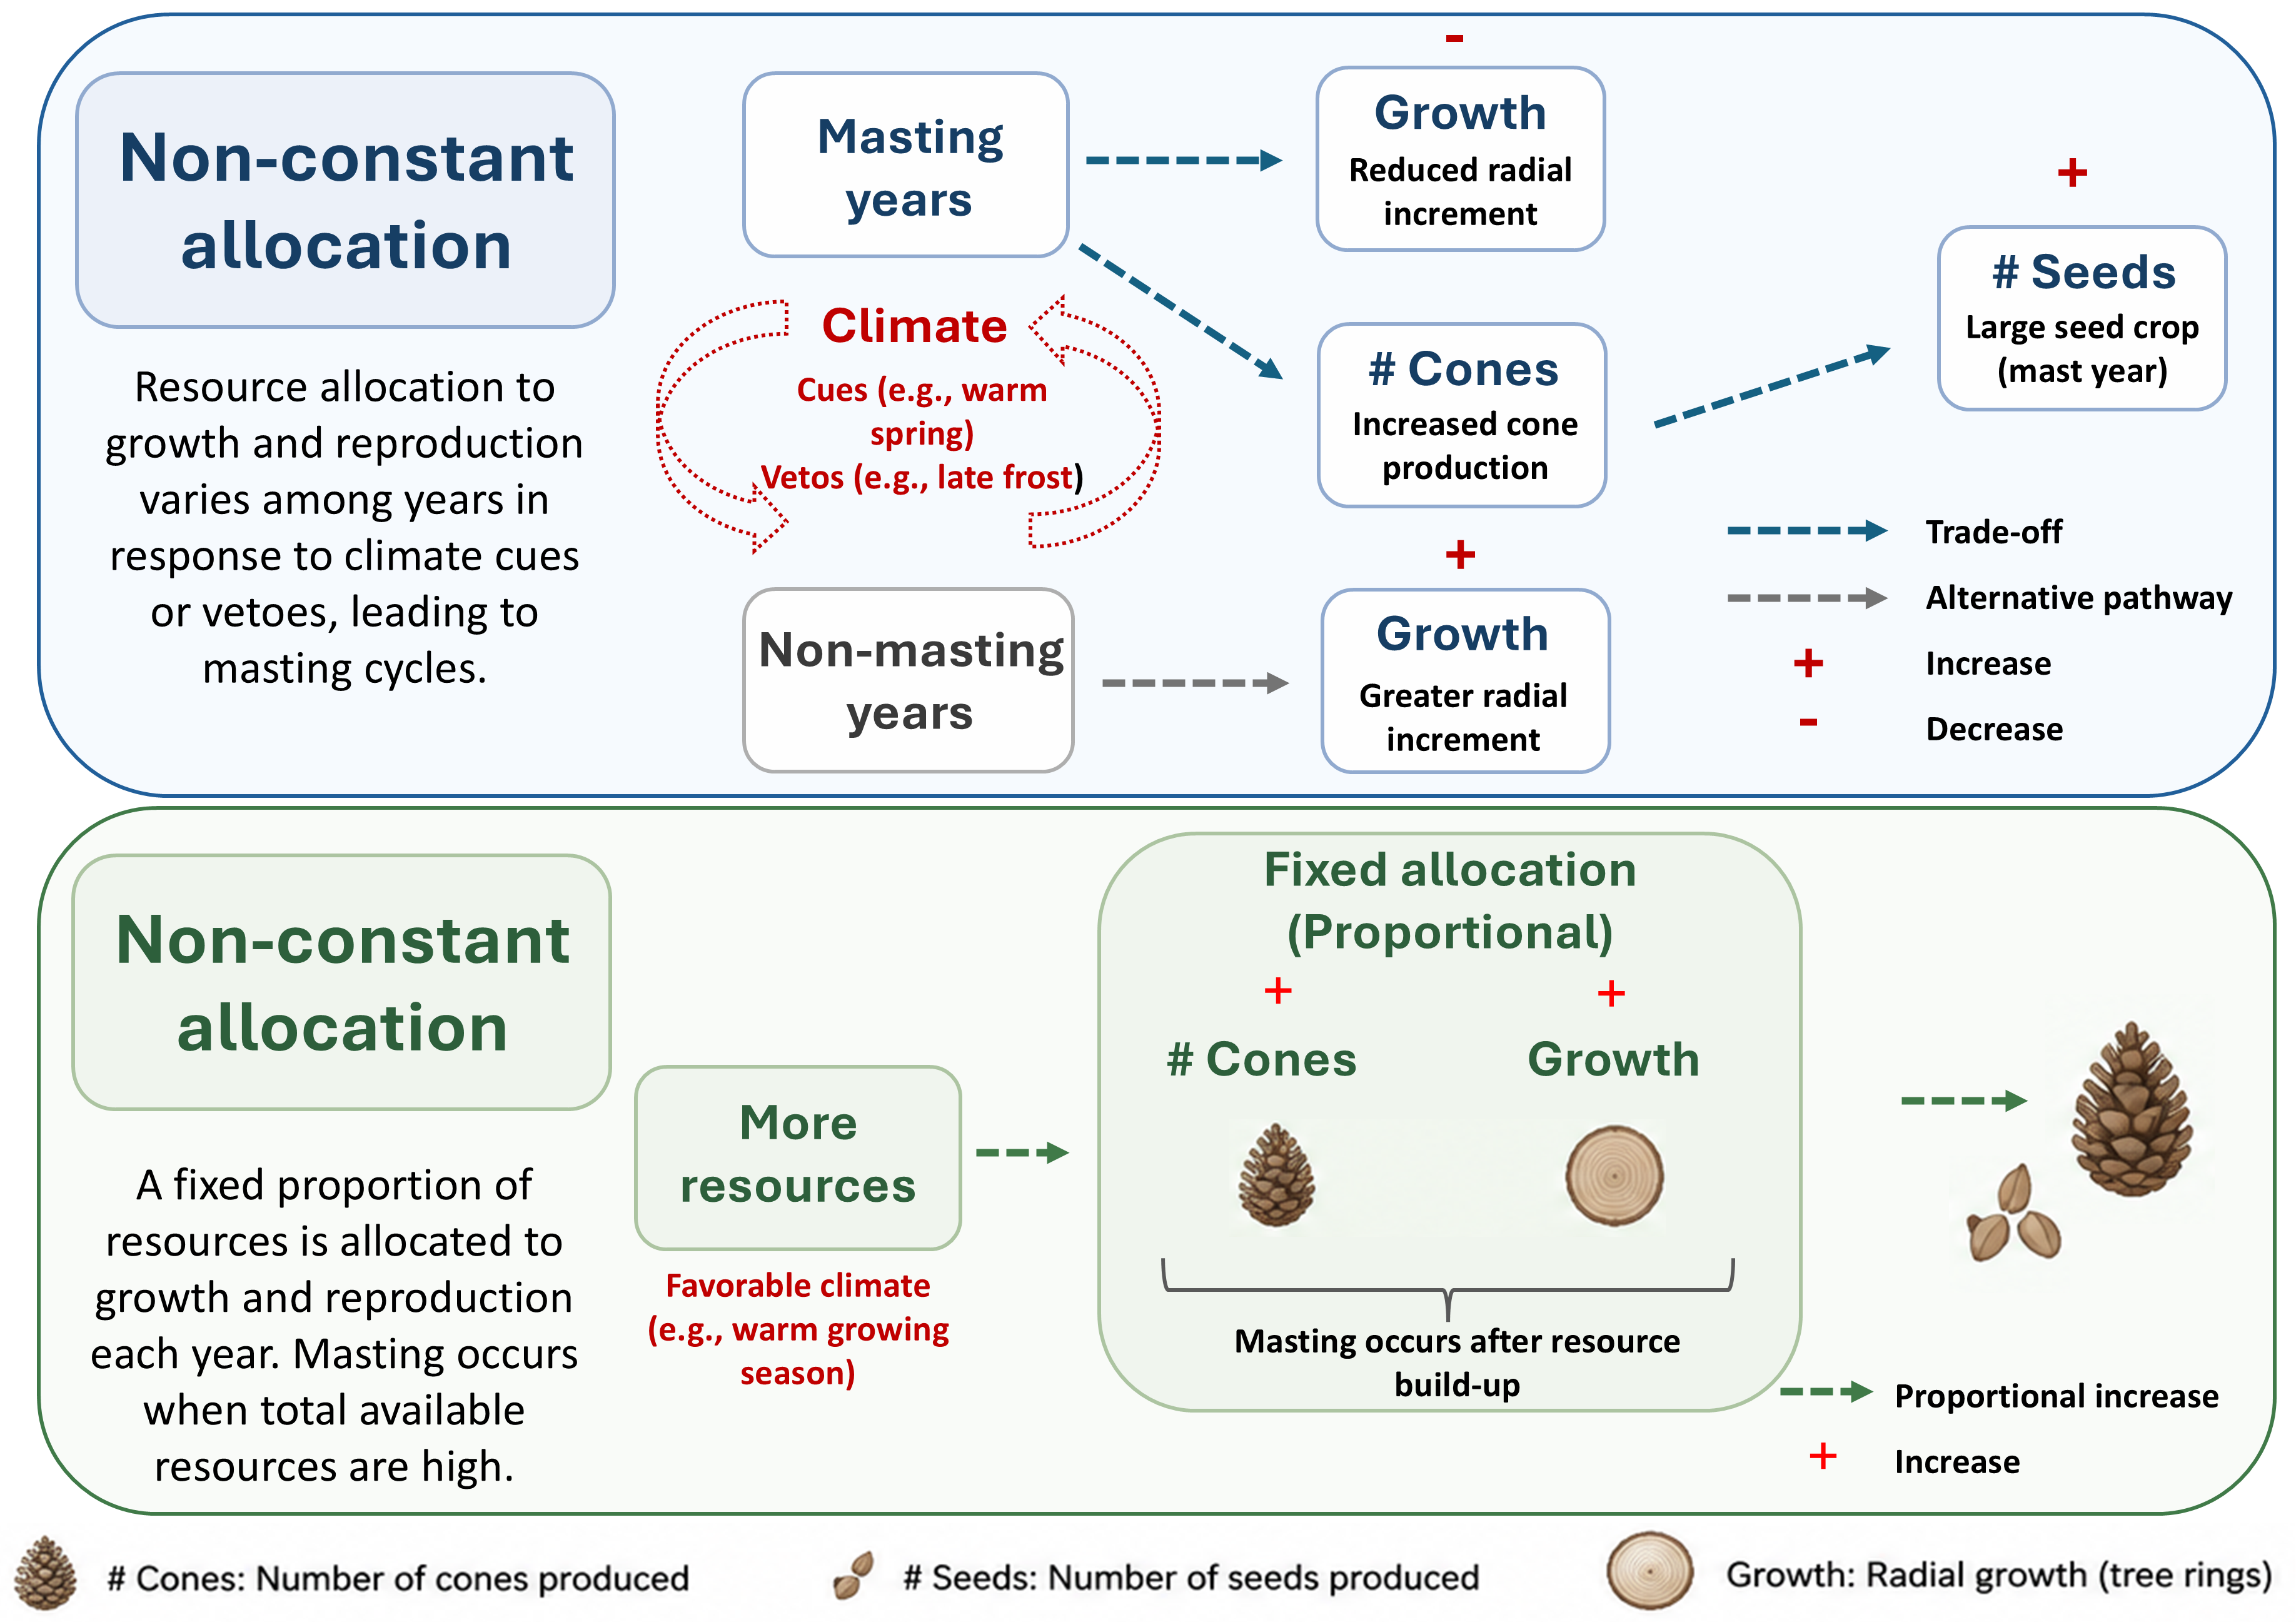
\includegraphics[width=\linewidth]{conceptualFigure.png}
    \setlength{\abovecaptionskip}{0pt}
    \caption{A conceptual figure showing constant and non-constant resource allocation to growth and reproduction.}
    \label{fig:cons}
\end{wrapfigure}
One hypothesis for masting, resource matching, suggests that a fixed fraction of resources is allocated to reproduction every year and masting occurs after enough resources have been accumulated \citep{kelly1994evolutionary}. (refer as `constant allocation in \ref{fig:cons}). However, the growth-reproduction trade-off  would suggest that increased investment in one process comes at the expense of the other \citep{grime1977evidence, stearns1998evolution}. It is more likely that allocation to growth and reproduction are non-constant and instead depend on environmental cues or environmental `vetos' \citep{hacket2016tree, pearse2016mechanisms} (refer as `non-constant allocation' in \ref{fig:cons}). Thus, it is important to understand the potential resources allocation strategy during a masting year or even in the years before and after as well as key climatic drivers behind these dynamics.

Masting concentrates reproduction into particular years, yet we do not know how strongly reproductive investment trades off against growth across years, whether this varies among species, or whether environmental conditions matters. This knowledge gap limits our ability to develop predictive models of masting that account for the physiological consequences of reproduction. In this proposed project, I will combine tree-ring and long-term seed trap data from two sites in the Pacific Northwest to quantify annual variation in growth and reproduction across six conifer species. I will address the central research question: \textbf{Is there a detectable trade-off between reproductive investment and growth, how does this relationship vary across species and environments, and how can this relationship improve predictions of future seed production under climate change?} My objectives are (1) to test whether increased reproduction is associated with reduced current or subsequent growth across elevation gradients in different species to identify which allocation strategy, constant or non-constant is supported in the context of masting and (2) to develop predictive models of seed production incorporating the empirically estimated allocation relationship to forecast future seed production under changing climate. I hypothesize that reproductive investment will reduce growth more strongly under environmentally stressful conditions, resulting a stronger growth-reproduction trade-off at higher elevations.

\textbf{Methods}
Although resource allocation cannot be measured directly over long time periods, annual radial growth and seed production provide complementary proxies for investment in vegetative growth and reproduction. We have already collected tree cores at Mount Tahoma, with a planned extension to Smithers, BC, where our lab has been collecting seedling data for several years. Together, these sites provide a broad latitudinal and environmental gradient that allows us to test how growth-reproduction relationships vary across environments and inform predictions of how masting may respond to future climate change\citep{hacket2021climate, korner2007use}. Many of the species are distributed across the sites, allowing us to build models that may work across the species range. Thus, conclusions from this study can potentially be extended to the broader Pacific Northwest and used to inform models that predict future growth and seed production.

We will combine:

\begin{itemize}
\item \textbf{Seed data} Long-term seed trap data (2008–present) collected by our collaborator Dr. Janneke Hille Ris Lambers, which records seed production by species across multiple forest stands.

\item \textbf{Growth data} We collected cores from targeted species in each stand with long-term seed data to assess the historical growth. Seed traps integrate seed production from multiple surrounding trees, so we sampled multiple individuals within the effective seed-trap catchment area and use stand/species-level hierarchical effects to account for this spatial aggregation. We targeted trees with DBH >25 cm to focus sampling on mature individuals with sufficient growth histories to overlap the seed-trap record.
\end{itemize}
%Tree core processing: I will prepare the cores for analysis by sanding them with fine grit sandpaper to ensure a smooth, clear surface. After preparation, I will scan the cores using a high-resolution camera to capture detailed images of the growth rings, then I will analyze the images with CooRecorder, a software used to measure tree ring width. I will also double check the cross-dating results with COFECHA, a computer program that assesses the quality of crossdating and measurement accuracy of tree-ring series \citep{cook2013methods, speer2010fundamentals}. All data will be uploaded to International Tree-Ring Data Bank once after processing.

Statistical analysis: I propose to use Bayesian hierarchical models to investigate the effects of current and lagged reproductive investment on annual radial growth. It partially pools estimates among species and elevations to allow for variation, while sharing information between groups to produce an overall estimate. The model will help determine whether the growth–reproduction trade-off is consistent across species, and whether it varies with elevation or environmental conditions. My next step will be a predictive model incorporating this relationship to create a more climate-sensitive model of mast seeding dynamics. This extended model will incorporate climate variables such as temperature and precipitation to assess how changing climatic conditions may alter the frequency, magnitude, and synchrony of mast seeding events.
	
\textbf {Significance}
We can gain insights into the adaptive strategies of different species along the environmental gradient and their potential resilience or vulnerability to future climate changes from the relationship between growth and reproduction regarding masting. All the species in this study are dominant tree species in Canada, which are not only ecologically significant but also economically important as key sources of timber. This knowledge could help us make more informed predictions about future forest dynamics, including shifts in species composition, regeneration, and ecosystem health in Canadian forests. As climate conditions continue to shift, understanding the masting behavior and growth responses will be important for effective forest management and conservation efforts, helping us to anticipate changes and make management plans that will support the sustainability and resilience of forest ecosystems.

\bibliographystyle{besjournals}
\bibliography{Proposal_NC} 
\end{document}
